\label{chap-it}

\citeb{Augustin2009} demonstrated the utility of a tensor product of a thin plate regression spline (for space) and a cubic spline (for time) in spatiotemporal smoothing. Using the soap film smoother described in chapter \ref{chap-intro} (in place of the thin plate spline), a spatiotemporal smooth is used to model the distribution of the incidence of the resident foreign population in Italy. This chapter presents the first application of this approach to spatiotemporal smoothing in a complicated geographic region. 

The work presented here is adapted from the article ``Modelling the spatiotemporal distribution of the incidence of resident foreign population in Italy'' by G. Marra (Statistical Science, University College London), D. L. Miller and L. Zanin (Prometia, Bolognia), accepted for publication in \textit{Statistica Neerlandica}. Each of the authors contributed equally to the article.

\section{Introduction \label{IN}}

\subsection{Background}

Many European countries have recently experienced a substantial increase in the proportion of immigrants in the population (\cite{Manning2010}). In particular this has increased since the introduction of new EU members in 2004 and 2007 (\cite{euexpansion}). 

Immigration statistics calculated at a national level do not provide information on the local spatial and temporal distribution of the phenomenon. This information may be of crucial importance for planning local policies. Using Italian data (at a municipal level) for the period 2003-2008, a tensor product smoother combining a cubic regression spline basis for time and a soap film spline basis for space can be used to create spatiotemporal maps. These maps could then be effectively used by policy makers to decide the allocation of economic resources at both a local and national level.

A \textit{municipality} (in Italian \textit{comune}) is the lowest level administrative sub-division in Italy. Municipalities then make up provinces (of which there are 110) which in turn make up regions (of which there are 20).

\subsection{Data}  

The \textit{resident foreign population} includes all people (born in Italy or abroad) who declare their citizenship not to be Italian. The change in resident foreign population at a municipal level, at the end of a year, is determined by
\begin{equation}
RFP^{31^\text{st}} = RFP^{1^\text{st}} + (I_1 + I_2 + I_3+ I_4) - (D_1 + D_2 + D_3 + D_4 + AC),
\label{it-rfp}
\end{equation}
where $RFP^{31^\text{st}}$ indicates the total number of resident foreigners at the end of December and $RFP^{1^\text{st}}$ the number of resident foreigners on the $1^\text{st}$ of January. $I_{1}$ denotes the number of people whose parents are foreigners (at least one of them being resident in the municipality), $I_{2}$ the number of foreign citizens who asked to transfer their residence from another Italian municipality to the current one, $I_{3}$ those who asked to transfer their residence from abroad, and $I_{4}$ refers to recording operations due to other reasons (e.g. foreigners mistakenly deleted from the registry of the municipality, because they were temporarily missing). $D_{1}$ represents the number of resident foreigners who died during the year, $D_{2}$ those who moved to a different municipality, $D_{3}$ those who moved abroad, $D_{4}$ refers to cancellations for other reasons (e.g. foreigners deleted from the registry of the municipality, because they were not present), and \textit{AC} denotes those resident foreigners who obtained Italian citizenship during the year. 

Given a specific area such as municipality (although this is often calculated on provincial, regional or national level too), a measure of density of resident foreign population is the percentage \textit{incidence of resident foreigners} (IRF), given as the ratio of the number of resident foreigners (the RFP) to the total resident population multiplied by 100 (e.g. \cite{Lowell2007}). This gives a simple demographic indicator for comparing different areas of a country in terms of number of resident foreigners per 100 resident inhabitants. According to ISTAT (the Italian government's statistical office), the IRF as calculated on a national level has grown substantially, from 2.7\% in 2002 to 6.5\% in 2008. 

Recently ISTAT has integrated the official statistics with a new public database (available via \url{http://demo.istat.it}), mainly based on administrative sources. The database gives the number of resident foreigners (calculated as above) in each of almost 8100 municipalities. Note that this does not include foreigners entering the country illegally, this issue is not addressed here. The quantification of illegal immigrants is an open topic of discussion in the studies of international migrations (e.g. \cite{Strozza2004}). Several approaches have been proposed in literature to quantify this, but all are subject to criticism (especially with regard to the magnitude of errors in estimates). Here only official data on the resident foreign population is considered. The ISTAT data, at a municipal level, (the highest resolution available at this time) is an excellent resource for creating maps.

\begin{figure}[tbp]
	\centering
		\includegraphics[width=\textwidth]{it/Raw}
	\caption{Empirical maps of the percentage incidence of resident foreigners in Italy over the years 2003-2008. These were obtained using ISTAT data at a municipal level.	The incidence is given as the ratio of the number of resident foreigners to the total resident population multiplied by 100. The colour scale ranges from an incidence of 0 (dark red) to an incidence of 12 (white).}
	\label{Rd}
\end{figure}

Figure \ref{Rd} shows plots of the raw IRF data at a municipal level over the years 2003-2008 (these are, of course, averaged over a grid for plotting purposes). The features that stand out clearly are the marked difference between north and south, and the increase in the IRF over time. However, these maps make it difficult to detect any local spatial structure in the incidence. For example, the Po Valley (northern Italy) has relatively high levels of IRF in 2008 but it is not really possible to clearly identify any particular areas of polarization. This can be problematic for policy makers in the central public administration who wish to allocate economic resources as efficiently and effectively as possible. Previous studies analysing the distribution of resident foreign population have employed descriptive analysis and/or to what amounts  to complex linear modelling approaches (e.g. \cite{Fonseca2008}, \cite{Longhi2010}). Using the soap film smoother, high resolution spatiotemporal maps of the IRF can be created.


\section{The model \label{METH}}

There are currently no relevant economic covariates available at a municipal level, the response (IRF) is modelled using a smoother which is a function of only the spatial coordinates and time. The model is then used to create smoothed maps of the geographical area of interest over time. Two points are noteworthy here. First, since the coastline of Italy has a complex boundary, leakage (as described in \secref{intro-FAS}) is likely to occur; inappropriately linking parts of the domain could have serious policy implications. Second, looking at figure \ref{Rd}, there appears to be a strong temporal interaction (those places with high incidence increase their incidence over time) so the model used should account for a space-time interaction. These two goals can be achieved by using a generalized additive model incorporating a three-dimensional tensor product smoother combining a cubic regression spline basis (\secref{intro-cubic}) for the temporal trend and a soap film smoother (\cite{soap} and \secref{intro-FAS}) for the spatial component.

\subsection{Model specification \label{MS}}

As explained in the introductory section, the IRF is given as the ratio of the number of resident foreigners to the total resident population multiplied by 100. The IRF may therefore only take positive values. Letting $f$ be a smooth function, the proposed model is as follows
\begin{equation}
\log \left\{\mathbb{E}(\texttt{irf}_{it})\right\} = f(\texttt{year}_t,\texttt{n}_i,\texttt{e}_i), \ \texttt{irf}_{it} \sim \text{Tweedie}\left\{\mathbb{E}(\texttt{irf}_{it}),\phi \mathbb{E}(\texttt{irf}_{it})^{p}\right\},          
\label{PropM}
\end{equation}
at municipality $i=1,\ldots,8094$ and year $t=2003,\ldots,2008$. $\phi$ is a dispersion parameter and the log link function ensures positive fitted values. $\texttt{irf}_{it}$, $\texttt{n}_i$, and $\texttt{e}_i$ represent the variables percentage IRF, Northing and Easting, respectively. Tweedie distributions are a special case of an exponential dispersion model and include, for example, the normal ($p=0$), Poisson ($p=1$) and gamma ($p=2$) distributions (\cite{Jorgensen}). For $1<p<2$ Tweedie distributions can be represented as Poisson mixtures of gamma distributions, with mass at zero but otherwise continuous on the positive reals. These are especially appealing for modelling continuous positive observations when exact zeros occur. \citeb{Dunn2005} provides a survey of published applications stressing the utility and flexibility of this class of distributions. $f$ is a multidimensional smooth function of \texttt{year}, \texttt{n} and \texttt{e} which models the joint effect of these variables on \texttt{irf}. Northing and Easting are as described in \secref{intro-basic-setup} (in this case the offsets used were 11.5 longitude, 44 latitude), thus ensuring that the spatial part of the smoother is isotropic (which would not be the case if latitude and longitude were used).

\begin{figure}[tb]
	\centering
		\includegraphics[width=3.5in]{it/pointmap.pdf}
	\caption{Raw data locations for the incidence of resident foreigners with the boundaries of Italy, Sardinia and Sicily. Each point is the location of the centroid of a municipality.}
	\label{pointmap}
\end{figure}

Note that the data were collected per municipality but enter into the model as points which are located at the centroids of the municipalities (see figure \ref{pointmap}). This change of support from areal to point data is not problematic and is desirable. The aim is to produce smoothed maps; using areal data would yield maps that are step functions for each municipality hence making it more difficult to see patterns in the data. To make the maps as easily interpretable as possible, smoothing of points is a clear choice.

The technical details of the construction of the smoothers is now covered. First, building on the general formulation given in \secref{GAMtensor}, the construction of a three-dimensional tensor product smoother is shown, using a one-dimensional temporal smoother and a two-dimensional spatial smoother. The details of the construction of the two-dimensional smoother, using the soap film smoother are then given. The final section details the construction of temporal trend estimates.

\subsection{A three-dimensional tensor product smoother for time and space \label{3D}}

The tensor product smooth used here is similar to the one shown in \secref{GAMtensor}, however it differs in two ways.  First, one of the components is a two-dimensional, isotopic spatial smooth ($f_\text{year}$) and the other component ($f_\text{space}$) is a marginal one-dimensional smooth of time. Second, the size of each basis is different.

Omitting the subscripts $i$ and $t$ for simplicity, the temporal smooth $f_\text{year}$ and spatial smooth $f_\text{space}$ can be written in terms of their basis decompositions (as in (\ref{intro-basisdecomp})):
\begin{equation*}
%f_\text{year}(\texttt{year})=\sum_{l=1}^L \xi_l b_l(\texttt{year})=\textbf{X}_\text{year}\bm\xi \ \ \text{and} \ \ f_\text{space}(\texttt{n},\texttt{e})=\sum_{r=1}^R \varphi_r d_r(\texttt{n},\texttt{e})=\textbf{X}_\text{space}\bm\varphi,
f_\text{year}(\texttt{year})=\sum_{j=1}^J \xi_j b_j(\texttt{year}) \ \ \text{and} \ \ f_\text{space}(\texttt{n},\texttt{e})=\sum_{r=1}^R \varphi_r d_r(\texttt{n},\texttt{e}),
\end{equation*}
where the $b_j(\texttt{year})$ and $d_r(\texttt{n},\texttt{e})$ are known cubic regression spline and soap film basis functions (respectively), with corresponding parameters $\xi_j$ and $\varphi_r$ and spline dimensions $J$ and $R$. 

In order to set up a three-dimensional tensor product smoother for time and space it is necessary for $f_\text{year}(\texttt{year})$ to vary smoothly with the spatial dimensions. This can be achieved by allowing the parameters $\xi_j$ to vary smoothly with \texttt{n} and \texttt{e}. Using the spline set-up for $f_\text{space}(\texttt{n},\texttt{e})$ we may write (analogously to \secref{GAMtensor}):
$$
\xi_j(\texttt{n},\texttt{e})=\sum_{r=1}^R \varphi_{jr} d_r(\texttt{n},\texttt{e}),
$$    
which results in:
$$
f(\texttt{year},\texttt{n},\texttt{e})=\sum_{j=1}^J \sum_{r=1}^R \varphi_{jr} d_r(\texttt{n},\texttt{e}) b_j(\texttt{year}). 
$$

To calculate the penalty, first let $J_\text{year}$ and $J_\text{space}$ be measures of the wigglyness of the functions $f_\text{year}$ and $f_\text{space}$ respectively. For $f_\text{year}$, the second-order cubic spline penalty evaluates $J_\text{year}(f_\text{year})=\int\left( \partial^2 f_\text{year}/\partial \texttt{year}^2 \right)^2 \text{d}\texttt{year}$ (\secref{intro-cubic}). The penalty for the soap film smoother used for the spatial part of the tensor product is covered in the next section; for ease of explanation it is treated as a black box here.

An overall penalty for the tensor product smoother can be obtained by applying the penalties of $f_\text{space}(\texttt{n},\texttt{e})$ to the varying coefficients of the marginal smooth $f_\text{year}(\texttt{year})$, $\xi_l(\texttt{n},\texttt{e})$,
$$
\sum_{j=1}^J J_\text{space}\left\{  \xi_l(\texttt{n},\texttt{e}) \right\},
$$ 
and the penalties of $f_\text{year}(\texttt{year})$ to the varying coefficients of the marginal smooth $f_\text{space}(\texttt{n},\texttt{e})$, $\varphi_r(\texttt{year})$,  
$$
\sum_{r=1}^R J_\text{year}\left\{  \varphi_r(\texttt{year}) \right\}.
$$ 
It follows that the penalty of $f(\texttt{year},\texttt{n},\texttt{e})$ can be written:
\begin{equation}
\lambda_\text{space} \sum_{j=1}^J J_\text{space}\left\{  \xi_l(\texttt{n},\texttt{e}) \right\} + \lambda_\text{year} \sum_{r=1}^R J_\text{year}\left\{  \varphi_r(\texttt{year}) \right\},
\label{it-fullpen}
\end{equation}
where as usual, $\lambda_\text{space}$ and $\lambda_\text{year}$ are the smoothing parameters for time and space respectively.

\Secref{intro-cubic} gives the details of the cubic spline basis used to model the temporal part of the smooth. The next section shows how $f_\text{space}$ and $J_\text{space}$ are constructed.

\subsection{The soap film smoother \label{SF}}

Since there is no particular reason to believe that the resident foreign population should be continuous across physical boundaries such as the Mediterranean Sea (at best there are merely potential resident foreigners in the sea), a smoother which takes into account of the fact that the borders of Italy represent both physical barriers should be used. Although there is no reason \textit{a priori} to believe that there will be particularly troublesome leakage (see \secref{intro-FAS}) here, mitigating against the issue by use of appropriate basis function choice from the outset is the most sensible course of action. 

As mentioned in \secref{intro-leakageapproaches}, the soap film smoother (\cite{soap}) uses a rather simple physical model to prevent leakage from occurring. First, consider the domain boundary to be made of wire, then dip this wire into a bucket of soapy water; a soap film with the same shape as the boundary will have then formed. Now consider the wire to lie in the $\texttt{n}$-$\texttt{e}$ plane and the height of the soap film at a given point to be the functional value of the model. This film is then distorted smoothly by moving it vertically toward each datum locally, while minimizing the surface tension in the film as a whole. Mathematically, the domain ($\Gamma$) is bounded by some polygon ($B$). For the islands of Sicily and Sardinia is their coastlines and for for the mainland is its coastline along with the border with France, Switzerland, Austria and Slovenia to the north. Note that a separate model was used for each of the mainland and Sardinia and Sicily (see \secref{ER} for why this was necessary).

The soap film smoother basis is quite similar in form to the thin plate regression spline basis given in \secref{GAMtprs}. The basis is split into two sets of functions to form a smoother that respect the necessary boundary conditions. The first basis is used for the smoothing within the region of interest, $\Gamma$; the second is to deal with the boundary, $B$. These two sets of basis functions are then summed to form:
\begin{equation*}
f_\text{space}(\texttt{n},\texttt{e})=\sum_{j=1}^J \alpha_j a_j(\texttt{n},\texttt{e}) + \sum_{k=1}^K \gamma_k g_k(\texttt{n},\texttt{e}),
\end{equation*}
where the $\gamma_k$ and $\alpha_j$ are the parameters to be estimated. One can think of the $a_j(\texttt{n},\texttt{e})$ as an offset dictated by the estimated boundary conditions on $B$ (similar to the linearly independent polynomials in the thin plate spline, although it is important to note that these functions are not planes) and the sum of the $g_k(\texttt{n},\texttt{e})$ as the smooth function to the data inside $\Gamma$ (analogous to the radial basis functions in the thin plate spline). Unlike thin plate splines however, the soap film basis requires the specification of $K$ knots inside $\Gamma$ and $J$ boundary knots on $B$ (here a grid is used for the internal knots and the boundary knots are equally spaced along $B$, further detail on the setup used is given in \secref{ER} and table \ref{soap-basis-table}). For convenience later, the second sum is labeled as $f_\text{int}$ (the part of $f$ with knots inside $\Gamma$). The rest of this section shows how these bases are constructed.

For the internal part of the smoother we first find a set of functions $\rho_k(\texttt{n},\texttt{e})$. These are each solutions to the Laplace's equation in two dimensions
$$
\frac{\partial^2\rho}{\partial \texttt{n}^2} + \frac{\partial^2\rho}{\partial \texttt{e}^2} = 0,
$$
except at one of the knots ($\texttt{n}^*_k,\texttt{e}^*_k$). Then, solving Poisson's equation in 2-dimensions
\begin{equation}
\frac{\partial^2 g_k}{\partial \texttt{n}^2} + \frac{\partial^2 g_k}{\partial \texttt{e}^2} = \rho_k(\texttt{n},\texttt{e}),
\label{soap-poisson}
\end{equation}
for $k$ indexing the $K$ knots. When the boundary condition $\rho_k(\texttt{n},\texttt{e})=0$ is applied, the set of basis functions for the soap film smoother $g_k(\texttt{n},\texttt{e})$ are found.  The partial differential equations (PDEs) are solved numerically using a multi-grid solver (e.g. \cite[pp. 862-880]{press1992numerical}), see the appendix of \cite{soap} for further technical details.

To find the height of the function at each point around the boundary a cyclic spline basis is used to construct $f_\text{bnd}(r)$. This $f_\text{bnd}(r)$ will have the expansion
\begin{equation}
f_\text{bnd}(r)=\sum_{j=1}^J \alpha_j \delta_j(r),
\label{soap-cyclic}
\end{equation}
where $r$ is the distance along the boundary, the $\alpha_j$ are parameters and $\delta_j(r)$ are cubic spline basis functions. The basis functions have the same form as the cubic spline discussed in \secref{intro-cubic}, but to ensure that the spline is cyclic the value of the function at the first knot is constrained to be the same as that at the last knot up to their second derivatives. Note that  the values of the $\alpha_j$ are not of interest at this stage, only the basis expansion. The basis functions $a_j(\texttt{n},\texttt{e})$ can be found by solving (\ref{soap-poisson}) for $\rho_k(\texttt{n},\texttt{e})= 0$ with the boundary condition resulting from setting $\alpha_j=1$ (and all other $\alpha_i$ to zero) in (\ref{soap-cyclic}), using the same methods as for the $g_k(\texttt{n},\texttt{e})$ above. Each $a_j(\texttt{n},\texttt{e})$ can then be thought of as the function with a peak at the corresponding knot on $B$, which are smooth across the whole of $\Gamma$.

The set of basis functions of $f_\text{int}$ have been found, as well as the boundary-induced-smooth which acts as a base for the soap film smoother. Although this seems like a rather esoteric setup, all the procedure above is effectively doing is setting up a basis such that standard penalized regression techniques can be used. Just as one might choose one spline basis over another for some property it possesses, the soap film basis has the property that it obeys the (estimated) boundary conditions of the region that are to be smoothed over.

In \secref{3D} the spatial penalty term was simply referred to as a single quantity, however (as was the case with the basis) the penalty is split into two parts: one for the cyclic smoother around the boundary and the other for the internal smoother. The easiest way to think about this is to write the spatial part of the penalty given in (\ref{it-fullpen}) as:
\begin{equation*}
\lambda_\text{space} \sum_{j=1}^J J_\text{space}\left\{  \xi_l(\texttt{n},\texttt{e}) \right\} = \lambda_\text{int} J_\text{int} + \lambda_\text{bnd} J_\text{bnd}.
\end{equation*}
The smoothing parameter $\lambda_\text{space}$ is not estimated and only exists as a way of making the tensor product explanation above clearer. The two interior and boundary penalties are now considered individually.

%Writing $\bm\beta$ as the vector of all smooth coefficients for the soap film, $\bm\gamma$ for the boundary parameters and $\bm\alpha$ for the interior, we have
%$$
%\bm\beta^\text{T}\textbf{S}^*_\text{space}\bm{\beta} = \lambda_\text{bnd} \bm\gamma^\text{T}\textbf{S}_\text{bnd}\bm{\gamma} + \lambda_\text{int} \bm{\alpha}^\text{T}\textbf{S}_\text{int}\bm{\alpha},
%$$
%where 
%$$
%\textbf{S}^*_\text{space} = \lambda_\text{bnd} \textbf{S}_\text{bnd} + \lambda_\text{int} \textbf{S}_\text{int}.
%$$
%$\textbf{S}^*_\text{space}$ is the total penalty for the spatial part of the smoother, $\textbf{S}_\text{int}$ is the interior penalty and $\textbf{S}_\text{bnd}$ is the cyclic spline boundary penalty. Both are matrices of known coefficients depending on the chosen basis functions. The $\lambda$ are the smoothing parameters for the boundary and interior smooth terms respectively. As in the previous section, for mathematical convenience, an asterisk indicates that the penalty matrices have been multiplied by the appropriate smoothing parameters. We now look at the two parts of the penalty individually. 

The isotropic interior penalty term is calculated as
$$
J_\text{int} = \int_\Gamma \Big(\frac{\partial^2 f_\text{int}}{\partial \texttt{n}^2}+\frac{\partial^2 f_\text{int}}{\partial \texttt{e}^2} 
\Big)^2\text{d}\texttt{n}\text{d}\texttt{e}.
$$
Note that the integration occurs only over $\Gamma$ rather than over the whole of $\mathbb{R}^2$ as would usually be the case. Also, there is no mixed derivative term, and the whole integrand is squared rather than each term individually (in contrast with, say, a thin plate regression spline penalty given in (\ref{tprs-pen})). This allows the $\texttt{n}$ and $\texttt{e}$ terms' derivatives to be traded off against each other so that the nullspace of the penalty is infinite dimensional. This permits those functions in the nullspace to be sufficiently wiggly to meet any boundary conditions. Note the similarity to the FELSPLINE penalty in \secref{intro-leakageapproaches}.

The penalty for the cyclic spline running about the boundary, used to estimate the $\alpha_j$, is calculated as 
$$
J_\text{bnd} = \int_B \Big(\frac{\partial^2 f_\text{bnd}}{\partial r^2}\Big)^2 \text{d}r.
$$
where the basis functions are the cubic regression splines defined above, but with the additional condition that the function's values and their first and second derivatives at the first and last knot must be equal. See e.g. \cite[p. 149]{simonbook} for more details.

The smooth function for $f_\texttt{space}$ obtained using the construction outlined above is rotationally invariant. Two smoothing parameters are estimated for the soap film (one for the interior and one for the boundary) but each controls the smoothness for both geographical directions at once (\cite{soap}). However, the tensor product smoother using the cubic regression spline basis for time and a soap film for space is not isotropic in space-time. This anisotropy is desirable since, as explained in Section \ref{MS}, the measurements of space and time are on different scales so it would not make sense to estimate one smoothing parameter for both the spatial and temporal components (e.g. \cite[p. 162]{simonbook}).
 
 In all, two smoothing parameters are estimated for the soap film ($\lambda_\text{int}$ and $\lambda_\text{bnd}$), and one for the temporal component ($\lambda_\texttt{year}$). Models were run using both REML and GCV for smoothness selection (with no major differences between the two methods). The results presented here are those for REML as described in \secref{intro-otherGAMfit}.
 
To summarize, the basis functions $a_j(\texttt{n}_i,\texttt{e}_i)$ and $g_j(\texttt{n}_i,\texttt{e}_i)$, and the penalties $J_\text{bnd}$ and $J_\text{int}$ have been found. Soap basis functions and penalties can be obtained using the the \textsf{R} package \texttt{soap} which implements the ideas discussed in this section.

\subsection{Variance and trend estimation \label{VE}}

Taking a Bayesian view it is possible to construct intervals using the posterior distribution of the model parameters. The interesting feature of these intervals is that, since they include both a bias and a variance component, they have good observed \textit{frequentist} coverage probabilities across the function (\cite{Marra2011}). The posterior distribution is given as
\begin{equation}
\bm\beta|\texttt{irf} \dot{\backsim} N( \hat{\bm\beta}, {\bf V}_{\bm\beta} ),
\label{Poster}
\end{equation}
where $\hat{\bm\beta}$ is the maximum penalized likelihood estimate of (all of) the smoother's parameters, $\bm\beta$ (i.e. concatenating all of the parameters discussed above into one vector). ${\bf V}_{\bm\beta}$ is of the form $(\mathbf{X}^\text{T}{\bf W}\mathbf{X}+{\bf S}^*)^{-1}\phi$, $\mathbf{X}$ contains the columns associated with the regression spline bases used to set up the model, ${\bf W}$ and $\mathbf{z}$ are the weight matrix and the pseudodata vector at convergence of the algorithm used to fit the penalized model and $\phi$ is the scale parameter (as in \secref{intro-extending-gams}). Given result (\ref{Poster}), confidence intervals for linear functions of the parameters can be found easily. Intervals for non-linear functions of the model coefficients can be conveniently obtained by simulation from the posterior distribution of $\bm\beta$. To aid interpretation of the results, trend estimates for some given areas of interest can be produced using the predictive distribution of $\texttt{irf}_{it}$, using the method proposed in \citeb{Augustin2009}. This approach can be implemented as follows:

\begin{enumerate}
	\item Repeat the following steps for $b=1,\ldots,N_b$, where $N_b$ represents the number of random draws. 
	   \begin{enumerate}
	      \item Simulate a random $N(\hat{\bm\beta}, \hat{{\bf V}}_{\bm\beta} )$ and call the resulting coefficient vector $\bm\beta_b$.
	      \item Calculate $\widehat{\mathbb{E}(\texttt{irf}_{it})}=\widehat{\texttt{irf}}_{itb}=\exp(\mathbf{X}^*_{it}\bm\beta_b)$, where $\mathbf{X}^*_{it}$ is evaluated at the observed values. 
	      \item For a given area of interest $a$ and year $t$, calculate
	      $$\widehat{\overline{\texttt{irf}}}_{tb}^a=\frac{1}{n_a}\sum_{i=1}^{n_a} \widehat{\texttt{irf}}_{itb},$$
	      where $n_a$ represents the number of observations in area $a$.     
	   \end{enumerate}
	\item Produce the required summary statistics, in this case median, lower and upper $95\%$ quantiles, for the temporal trend $\widehat{\overline{\texttt{irf}}}_{tb}^a$.
\end{enumerate}
Small values for $N_b$ are typically tolerable. In practice, $N_b$ can be set to $100$. Increasing this value does not change the results which are presented in the next section.
 

\section{Results \label{ER}}

The model was implemented using the basis sizes (for the cubic and cyclic regression splines) and interior knots (for the soap film) given in table \ref{soap-basis-table}. Note that separate models were used for each of mainland, Sicily and Sardinia since scenarios with multiple islands are not currently supported in the \texttt{soap} package.

\begin{table}[t]
\centering
\begin{tabular}{c c c c}\\
Region & Interior knots & Cyclic spline basis size & Cubic spline basis size\\
\hline
Mainland & 41 ($14 \times 14$) & 20 & 6\\
Sardinia & 12 ($5 \times 6$) & 8 & 6\\
Sicily & 12 ($6 \times 6$) & 10 & 6\\
\end{tabular}
\caption{Basis sizes per region for the smooth functions to be fitted to the Italian data. For the interior (soap film) knots, the numbers in brackets show the initial grid, the other number gives the number of knots actually used (those inside the boundary).}
\label{soap-basis-table}
\end{table}

The parameter for the Tweedie distribution ($p$ in (\ref{PropM})) was set to $1.2$. It was chosen by trial and error to produce the best possible residual plots. The estimate for $\phi$ was equal to $0.905$. Before employing the class of Tweedie models, simpler gamma distribution-based models were used; diagnostic plots suggested the presence of substantial structure in the residuals. Residual analysis was carried out following an approach similar to that of \citeb{Chandler2005}. Figure \ref{Resid} gives some diagnostics for the proposed model. Overall, the first two sets of boxplots do not show long-term trends, but suggest the presence of some spatial residual structure. The normal Q-Q plot shows some curvature in the upper tail. The scale-location plot indicates the presence of some heteroskedasticity, although the LOESS smooth running though the plot (grey line) does not indicate a relationship between absolute residuals and predicted values. The presence of extreme values in all diagnostic plots suggest under-estimation of the IRF on occasion. Descriptive analysis revealed that some municipalities have considerably higher IRF levels compared to those in neighbouring municipalities. This is mainly due to the specific socio-economic features of attractiveness of each municipality which need to be accounted for in order to avoid under-estimation. Unfortunately, as pointed out in the introduction, currently no relevant economic data are available at a municipal level and hence such information can not be incorporated in the model. The deviance explained was 57\%. 

As a check, the proposed model was fitted again but replacing the response variable with the residuals. The resulting maps suggested the presence of some residual structure in those municipalities characterized by very high IRF levels; this was expected given the presence of extreme residuals evidenced in the diagnostic plots. Sensitivity analysis showed that the results do not change if more basis functions are used for the smooth term in the model. 

\begin{figure}[tbp]
	\centering
		\includegraphics[width=0.75\textwidth, angle=270]{it/Resid.eps}
	\caption{Deviance residual diagnostics from the spatiotemporal model of the incidence of resident foreigners. Row-wise from top: (i) yearly distributions, (ii) distributions of residuals grouped according to squares on a 10x10 grid which fell inside the boundary, (iii) normal Q-Q plot, (iv) absolute residuals versus predicted values, with LOESS curve (grey line).}
	\label{Resid}
\end{figure}

The proposed model was compared with one in which the spatial and temporal effects were simply additive. As in \citeb{Augustin2009}, Schwarz's Bayesian Information Criterion (BIC, see e.g. \cite[p. 286]{burnhamanderson}) was used to compare the two models; the latter yielded an increased BIC. Visually comparing the maps produced by these two models, the proposed model contained details that could not be seen in the model where the spatial and temporal effects were additive.

Despite the lack of fit corresponding to those municipalities characterized by very high levels of the IRF, the analysis above suggests that the proposed model is able to capture the overall spatiotemporal structure present in the data. Should some relevant economic variables become available at a municipal level, the model specification and, as a consequence, its explanatory power could be considerably improved. 

\subsection{Spatiotemporal maps \label{STT}}

As mentioned in the introductory section, Italy's national IRF was 6.5\% in 2008. Obviously, this number says nothing about specific local areas with particularly high or low levels of resident foreigners. Moving to smaller aggregations (say, the regional or provincial level) the same argument holds: some information is lost. This kind of low resolution statistic can mask smaller-scale heterogeneity in the population. Our aim here is to capture exactly this spatial heterogeneity.

At first glance, figure \ref{Rd} shows the stark contrast between north and south. The maps also highlight the inhomogeneous spatial and temporal distribution of the IRF. However, as pointed out above, smoothed maps can give a much better picture of the distribution of the IRF. Smoothing the maps allows for the separation of signal and noise in the data, giving an idea of the overall structure of the phenomena, as well as providing a trend information via a temporal component of the model. Figure \ref{it-fig1} shows smoothed spatiotemporal maps of the IRF in Italy for the period 2003-2008, obtained using the approach described in the previous sections. The maps show that in 2003 northern and central Italy have the highest levels IRF. Over the subsequent years (2004-2008), the incidence spreads, forming four main areas where resident foreigners tend to live. Focusing on 2008, the most popular areas are in north Italy, specifically the Emilia-Romagna and Lombardy regions (with captials Bologna and Milan, respectively). These, although popular in 2003, appear to have increased their incidence. The second most attractive area is made up of the central Italian regions of Tuscany, Umbria, Marche and Lazio. The final two areas are composed of Liguria and Piedmont, and Veneto, Friuli-Venezia Giulia and Trentino-Alto Adige, in the northwest and northeast of the country, respectively. There is also an interesting growth in the incidence at the Swiss and Austrian borders (from about 2\% in 2003 to about 4-5\% in 2008). Resident foreigners seem less attracted by the regions and islands of southern Italy. Returning to the Po Valley area, the maps in figure \ref{it-fig1} allow us to identify the presence of two large, well defined polarization patterns in the IRF, the first in the centre of the Po Valley and the second near Venice. The maps in figure \ref{Rd} do not reveal these patterns.

\begin{figure}[t]
	\centering
		\includegraphics[width=\textwidth]{it/maps-Soap.pdf}
	\caption{Spatiotemporal maps of the percentage incidence of resident foreigners in Italy over the years 2003-2008. These were obtained using model (\ref{PropM}) with a tensor product smoother based on a cubic regression spline basis for time and a soap film spline basis for space, and ISTAT data at a municipal level. Predictions were made over those points lying inside the study region from a 100 by 100 grid. The incidence is given as the ratio of the number of resident foreigners to the total resident population multiplied by 100. The colour scale ranges from an incidence of 0 (dark red) to an incidence of 12 (white). Blue lines indicate contours separated by a one unit change in incidence.}
	\label{it-fig1}
\end{figure}

Figure \ref{trends} shows the estimated temporal trends for both the full Italian territory and broken down by area with 95\% confidence intervals (using the approach in \secref{VE}). The trends for northern and central Italy are similar. However, those for southern Italy and the islands are much flatter. Northern and central Italy also show a faster growth in incidence. Such differences are supported by the confidence intervals. Overall, these trends reflect what we see in the maps in figure \ref{it-fig1}, that there is a significant difference between northern/central Italy and the south of the country and its islands. Note that, since the approach outlined in \secref{VE} cannot account for the presence of residual correlation structure, one would expect the obtained confidence intervals not to be exactly representative than those that might be produced when adjusting for such correlation. The most obvious approach would be to fit a generalized additive mixed model (\cite[chapter 6]{simonbook}) with a carefully chosen correlation structure. Unfortunately convergence problems prevented such a model from being fitted.

\begin{figure}[t]
	\centering
		\includegraphics[width=\textwidth]{it/trends.pdf}
	\caption{Temporal trends in incidence of resident foreigners over the study period for Italy (top left), followed by trend estimates for north, central and south and islands areas with 95\% confidence intervals. North was defined as those points in the prediction grid above -20 km north, central as between -20 km and -300, and south and islands (including Sardinia and Sicily) as below -300.}
	\label{trends}
\end{figure}

The results presented in this section can be useful for policy-makers who may want to allocate economic resources as efficiently and effectively as possible, supporting, for instance, policies and services needed for the integration of resident foreigners. Such policies relate to a number of services such as: admission to education, access to the public health service, professional training, services supporting the match of labor supply and demand. For sociologists and demographers these maps may represent a new way to model spatiotemporal demographic changes and display the results graphically. 

\section{Conclusions}
\label{it-conc}

This chapter has shown an application of the soap film smoother as part of a larger spatiotemporal model. It has also hopefully shown that the models defined in chapter \ref{chap-intro} can be usefully applied to spatial smoothing as well as illustrating the modelling process.

The smoothed maps show in figure \ref{it-fig1} and the trends in figure \ref{trends} show that modelling the incidence of resident foreigners properly can give a much better picture of the distribution of the IRF as compared to just looking at the empirical maps in figure \ref{Rd}. The maps clearly show which parts of Italy are more popular with resident foreigners and the temporal trends gave an indication of the differences between different areas over time (in particular north and south). This information may be crucial for policy-makers who may want to allocate economic resources as efficiently and effectively as possible for supporting (for example) policies and services needed for the integration of resident foreigners.

Should some relevant economic variables become available at a municipal level, logical extensions incorporating covariate effects could be considered. This might assist in determining what further factors affect the distribution of resident foreigners in Italy and further aid decision making.

Using a tensor product of the soap film with the cubic regression splines allowed for the full interaction between the spatial and temporal components of the model. This approach is relatively simple to implement thanks to the ease of developing such models using the \textsf{R} packages \texttt{mgcv} and \texttt{soap}. There were, however, some difficulties. Specifically, it was not possible to build a model for both the mainland and islands simultaneously, which would allow for the estimation of a single temporal smooth for the whole of the country. It is also unfortunate that it was not possible to fit a generalized additive mixed model to take into account the correlation in the data, this was due to numerical issues (in particular the optimization procedure failed to converge).

This analysis has given some idea of the practical considerations from the point of view of an investigator when smoothing over regions with complex boundaries. Being able to code models in a familiar environment makes the process of developing a model much easier (writing the model definition in \textsf{R} for the model used here is only marginally more complicated than that for a more standard GAM). Keeping within the GAM framework allows for the usual diagnostic procedures to be used, making model checking straightforward. On an extremely practical level, it was apparent that the amount of time that it takes to fit the model becomes a serious consideration during development; waiting for models to fit or to fail to converge can cause frustration and only acts as a barrier to wide-adoption. The methods developed in the coming chapters should take this into account.


